\begin{figure}[h!]
    \centering
    
    % =======================
    % Row 1 — Input
    % =======================
    \begin{minipage}{0.08\columnwidth}
        \centering
        \rotatebox{90}{\small Input}
    \end{minipage}
    \begin{minipage}{0.25\columnwidth}
        \centering
        
\includegraphics[width=\textwidth]{puppy-pi/rs/frame55.png}
    \end{minipage}
    \begin{minipage}{0.25\columnwidth}
        \centering
        
\includegraphics[width=\textwidth]{puppy-pi/rs/frame92.png}
    \end{minipage}
    \begin{minipage}{0.25\columnwidth}
        \centering
        
\includegraphics[width=\textwidth]{puppy-pi/rs/frame90.png}
    \end{minipage}

    \vspace{1mm}

    % =======================
    % Row 2 — Prediction
    % =======================
    \begin{minipage}{0.08\columnwidth}
        \centering
        \rotatebox{90}{\small Prediction}
    \end{minipage}
    \begin{minipage}{0.25\columnwidth}
        \centering
        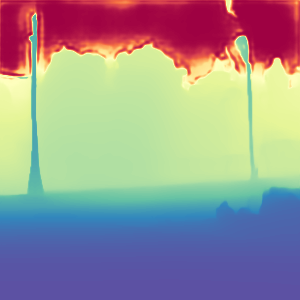
\includegraphics[width=\textwidth]{puppy-pi/depth/rs/frame55_pred.png}
    \end{minipage}
    \begin{minipage}{0.25\columnwidth}
        \centering
        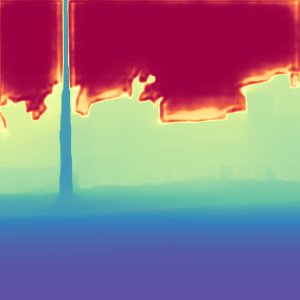
\includegraphics[width=\textwidth]{puppy-pi/depth/rs/frame92_pred.png}
    \end{minipage}
    \begin{minipage}{0.25\columnwidth}
        \centering
        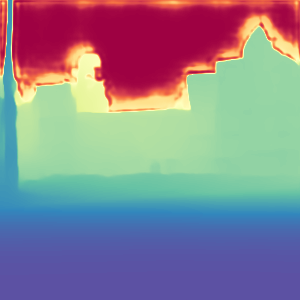
\includegraphics[width=\textwidth]{puppy-pi/depth/rs/frame90_pred.png}
    \end{minipage}

    \vspace{1mm}

    % =======================
    % Row 3 — Ground Truth
    % =======================
    \begin{minipage}{0.08\columnwidth}
        \centering
        \rotatebox{90}{\small Ground Truth}
    \end{minipage}
    \begin{minipage}{0.25\columnwidth}
        \centering
        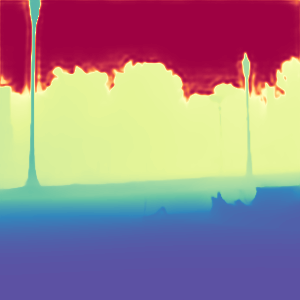
\includegraphics[width=\textwidth]{puppy-pi/depth/gs/frame55.png}
    \end{minipage}
    \begin{minipage}{0.25\columnwidth}
        \centering
        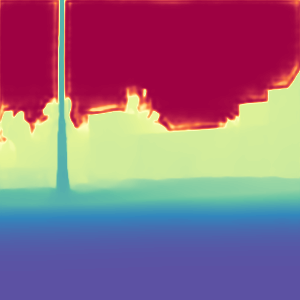
\includegraphics[width=\textwidth]{puppy-pi/depth/gs/frame92.png}
    \end{minipage}
    \begin{minipage}{0.25\columnwidth}
        \centering
        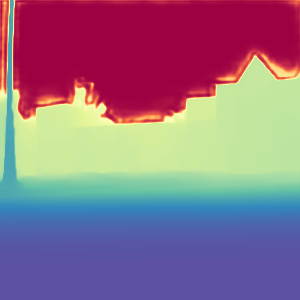
\includegraphics[width=\textwidth]{puppy-pi/depth/gs/frame90.png}
    \end{minipage}

    \caption{
    Visualization of condensed model run on Puppy-Pi data. Rolling shutter effects manifest in the angles of light poles being non-vertical, and corrected to be properly angled when ran through the model.
    }
    \label{fig:puppy}
\end{figure}